\chapter{Uso del sistema \label{sec:usodelsistema}}
Este apartado esta destinado a explicar los pasos y comandos necesarios para poner en marcha el sistema \textit{bigdata} implementado en el apartado \ref{sec:implementación} y poder utilizarlo. Por tanto, se explicarán los scripts y comandos necesarios para realizar la conexión de los nodos y establecimiento de los clúster, así como los necesarios para ejecutar las funciones del sistema y, finalmente, se analizarán los scripts utilizados para realizar las pruebas.

\section{Arranque de las máquinas}
En este apartado hay que diferenciar entre los dos modos de ejecución disponibles, el modo pseudo-distribuido y el distribuido. Para el primero, este paso solo consiste en el encendido de la máquina a utilizar.

En el caso del segundo, el proceso es más complejo, ya que, además de encender cada uno de los nodos, hay que comprobar que su conexión a la red es correcta, es decir, se tiene que verificar que el equipo esté conectado a la red y que la configuración de las direcciones IP y los nombres de red es correcto.

Además, en este segundo caso, también hay que comprobar que las conexiones \gls{SSH} se realizan correctamente entre los nodos.

\section{Arranque de \textit{Apache Spark} \label{arranqueSpark}}
Este paso solo será necesario realizarlo en el caso de los sistemas distribuidos, ya que el modo pseudo-distribuido solo contiene un nodo, por lo que no hay que establecer ningún tipo de conexión, necesitando solo el envío de un trabajo para su funcionamiento.

En el caso del modo multinodo, el proceso de inicialización de \textit{Apache Spark} se realiza ejecutando un script contenido en la carpeta donde está instalado el \gls{framework}. Este ejecutable, que se encuentra en la ruta ``\$HOME/bigdata/spark/sbin/start-all.sh'', será el encargado de realizar las conexiones con los nodos esclavos y arrancar la interfaz web de \textit{Apache Spark}, que se puede apreciar en la figura \ref{fig:interfazSpark}.

Este script se ejecutará desde el nodo maestro. En cuanto a la interfaz web, nos permitirá comprobar que todos los nodos están conectados correctamente y, además, el estado de los trabajos que está realizando o ha realiza el sistema.

\begin{figure}[htp!]
\centering
\caption{Interfaz web de \textit{Apache Spark}}
\label{fig:interfazSpark}
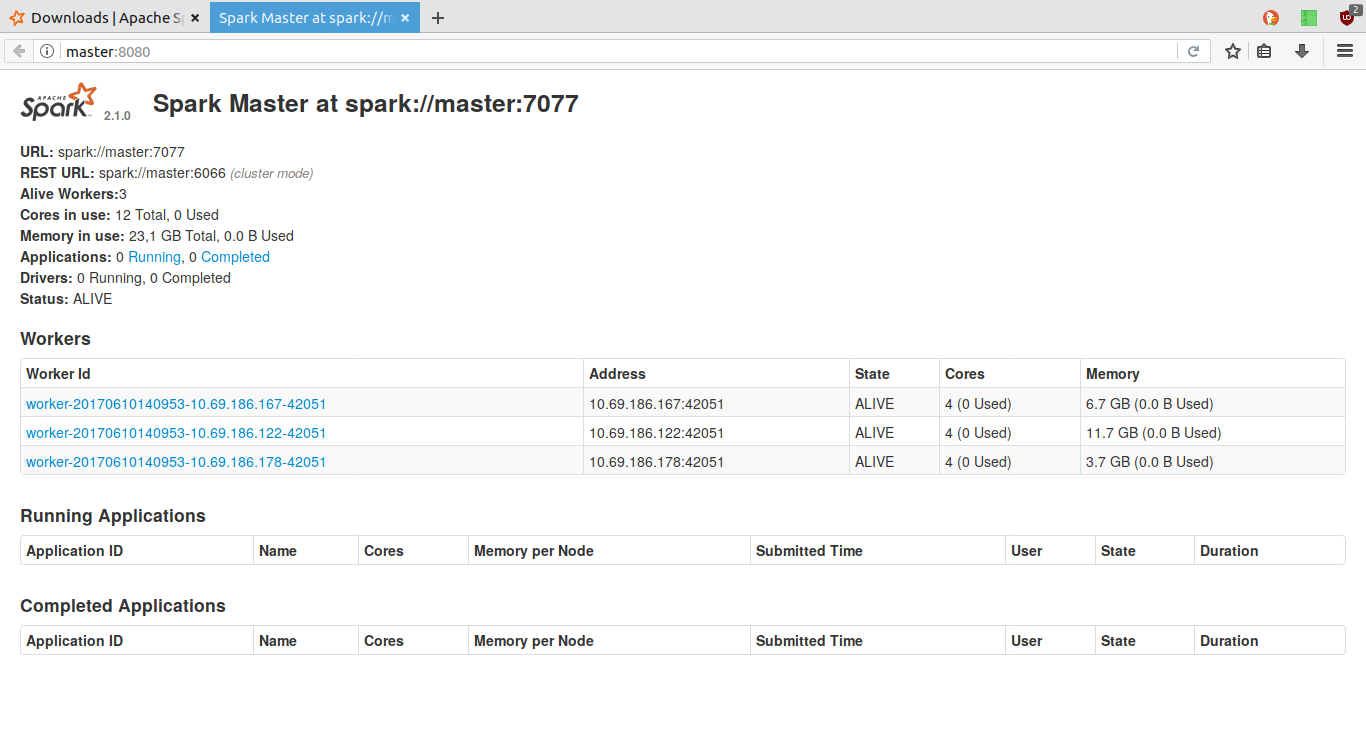
\includegraphics[scale=0.3]{graphics/clusterDom}
\end{figure}

\section{Arranque de \textit{Apache Hadoop}}
Como se indicó en los apartados \ref{disDomestico} y \ref{hadoopClusterDom}, la arquitectura \textit{big data} contará con el sistema de replicación de \textit{Apache Hadoop} únicamente en la configuración multinodo doméstica. En este apartado, se tratará el arranque y parada del \gls{HDFS}, además de otros comandos para su manipulación.

De forma muy similar a \textit{Apache Spark}, el arranque del sistema de replicación se realiza mediante un script que está contenido en la carpeta de instalación, en la ruta ``/\$HOME/bigdata/hadoop/sbin/start-dfs.sh''. Este ejecutable se encarga de arrancar del sistema de replicación en todos los nodos, realizando la transmisión de los datos si es necesario desde el maestro a los nodos.

Para parar el sistema, también se cuenta con un script encargado de detener el sistema de replicación y realizar la desconexión entre los equipos. Este se encuentra en ``/\$HOME/bigdata/hadoop/sbin/start-dfs.sh''. Con respecto al resto de comandos, estos se comentarán en el fragmento de código \ref{comandosHDFS}.

\begin{lstlisting}[label=comandosHDFS,language=sh,frame=single,caption=Comandos \textit{Apache Hadoop}]
# Formatear sistema de replicacion
hdfs namenode -format

# Crear carpeta en el sistema
hdfs dfs -mkdir /nombreCarpeta

# Copiar desde local al sistema de replicacion
hdfs dfs -put /rutaLocal /rutaHDFS

# Eliminar archivo o carpeta del sistema de replicacion
hdfs dfs -rmr /rutaParaEliminar
\end{lstlisting}

Este sistema de replicación también contará con una interfaz web que alojará el nodo maestro, en ella se podrá comprobar el estado de cada nodo y navegar por el sistema de ficheros. Ambas funciones se pueden apreciar en las figuras \ref{fig:compHadoop} y \ref{fig:fichHadoop}.

\begin{figure}[htp!]
\centering
\caption{Interfaz web de \textit{Apache Hadoop} con el estado de los nodos}
\label{fig:compHadoop}
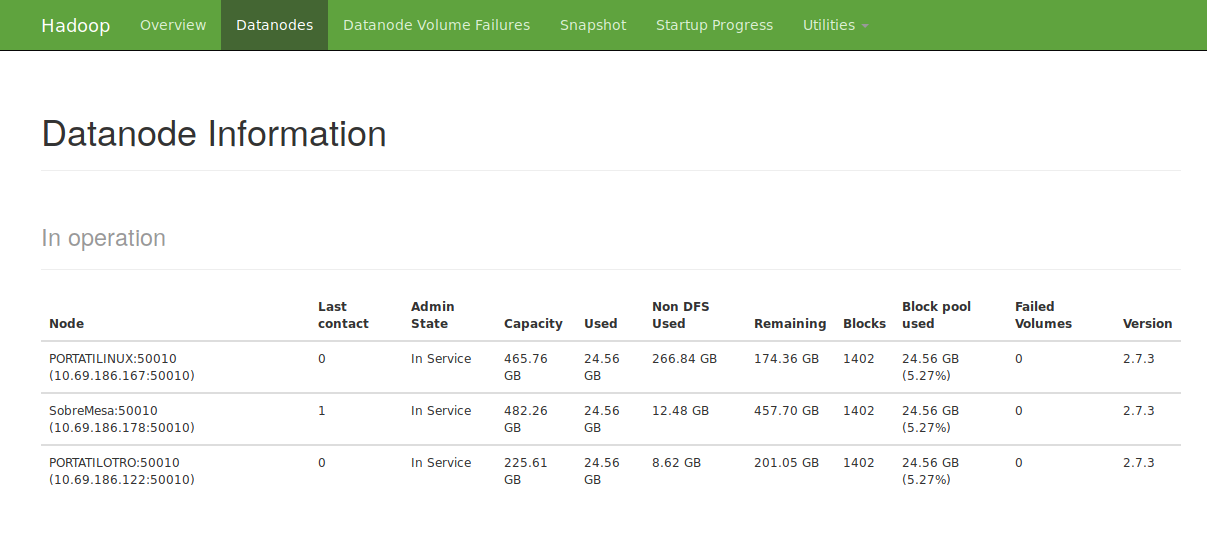
\includegraphics[scale=0.35]{graphics/hadoopDatanode}
\end{figure}

\begin{figure}[htp!]
\centering
\caption{Interfaz web de \textit{Apache Hadoop} con el navegador del sistema de ficheros}
\label{fig:fichHadoop}
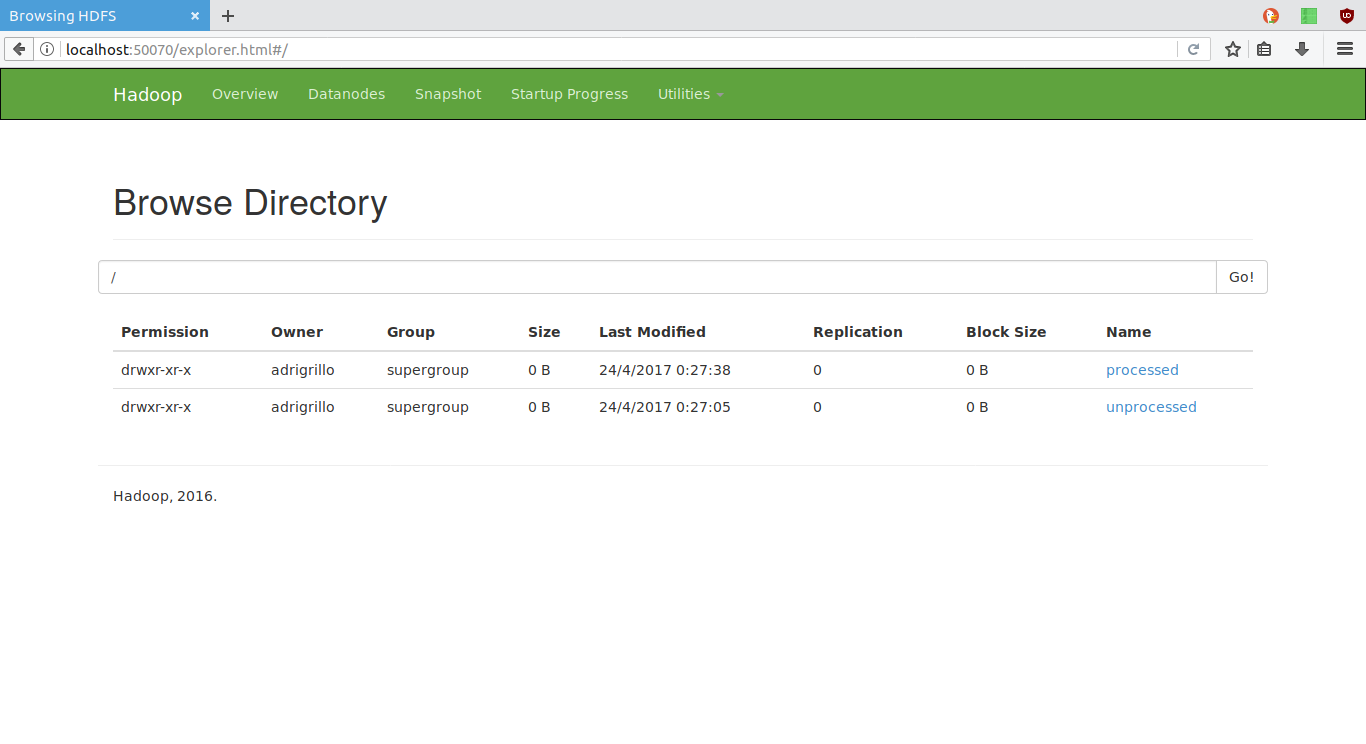
\includegraphics[scale=0.35]{graphics/directorioHadoop}
\end{figure}

\section{Ejecución de trabajos en \textit{Apache Spark}}
Para ejecutar un trabajo de \textit{Apache Spark} se utilizará el script ``spark-submit'' que es el que se encargará de gestionar el proceso. Este ejecutable se localiza en la ruta ``/\$HOME/bigdata/spark/bin/spark-submit'' y, entre otros argumentos \cite{submitSpark}, hay que introducir la clase con el código del trabajo a ejecutar y, si es necesario, la dirección web del maestro del clúster, para que este reparta el trabajo. En el fragmento de código \ref{submits} se mostrará la forma de enviar un trabajo dependiendo de la configuración de la arquitectura.

\begin{lstlisting}[label=submits,language=sh,frame=single,caption=Comando para el envío de un trabajo a \textit{Apache Spark} dependiendo del modo de ejecución de la arquitectura \textit{big data}]
# Submit en el modo pseudo-distribuido
/$HOME/bigdata/spark/bin/spark-submit fichero.py

# Submit en el modo distribuido
/$HOME/bigdata/spark/bin/spark-submit --master spark://nombreRedMaestro:7077 fichero.py
\end{lstlisting}


\section{Ejecución del procesado de datos}
El componente del procesado de los datos está contenido en la clase ``DataProcessing.py'', que se encuentra en la carpeta destinada al guardado del código fuente y los scripts, en la ruta ``/\$HOME/bigdata/src/DataProcessing.py''.

Esta clase será la encargada de la limpieza y el tratamiento de los registros, como se ha explicado en el apartado \ref{anaProcData}. Este fichero se ejecutará desde la terminal y tomará tres argumentos para su correcto funcionamiento, que serán los siguientes:

\begin{itemize}
\item \textbf{Fichero:} Fichero de datos sin procesar sobre los que trabajar. Este nombre tiene que coincidir con algún fichero de la carpeta ``unprocessed'', sin introducir la extensión \textit{*.csv}.
\item \textbf{Nombre:} Nombre del archivo con el que se desea guardar el resultado del procesamiento, en general, se utilizará el nombre del fichero a procesar.
\item \textbf{Tiempos:} Nombre con el que se desea guardar el archivo que contendrá el tiempo de procesamiento de la ejecución.
\end{itemize}

\section{Ejecución de las consultas}
Los ficheros que contienen el código de las consultas, al igual que el fichero de procesamiento, se encuentran en la ruta ``/\$HOME/bigdata/src/''. En este caso, para cada consulta habrá una clase de Python, estas serán:

\begin{itemize}
\item \textbf{FrequentRoutes.py:} Rutas más frecuentes sin estacionalidad. Los argumentos de entrada son:
\begin{enumerate}
\item \textbf{Fichero:} Fichero sobre el que se realizará la consulta, coincidente con alguno de la carpeta ``processed''.
\item \textbf{Fecha:} Día, mes y año sobre el que se trabajará, \textit{string} con el formato ``aaaa-mm-dd''.
\item \textbf{Hora:} Hora y minutos sobre la que establecer la ventana de tiempo, \textit{string} con el formato ``HH:MM''.
\end{enumerate}

\clearpage
\item \textbf{FrequentRoutesDay.py:} Rutas más frecuentes con estacionalidad.
\begin{enumerate}
\item \textbf{Fichero:} Fichero sobre el que se realizará la consulta, coincidente con alguno de la carpeta ``processed''.
\item \textbf{Mes:} Nombre del mes al que se le quiere dar más valor para calcular la influencia de los registros.
\item \textbf{Día de la semana:} Día de la semana sobre la que se trabajará.
\item \textbf{Hora:} Hora y minutos sobre la que establecer la ventana de tiempo, \textit{string} con el formato ``HH:MM''.
\end{enumerate}

\item \textbf{ProfitableAreas.py:} Zonas que más beneficios proporcionarían al taxista sin estacionalidad.
\begin{enumerate}
\item \textbf{Fichero:} Fichero sobre el que se realizará la consulta, coincidente con alguno de la carpeta ``processed''.
\item \textbf{Fecha:} Día, mes y año sobre el que se trabajará, \textit{string} con el formato ``aaaa-mm-dd''.
\item \textbf{Hora:} Hora y minutos sobre la que establecer la ventana de tiempo, \textit{string} con el formato ``HH:MM''.
\end{enumerate}

\item \textbf{ProfitableAreasDay.py:} Zonas que más beneficios proporcionarían al taxista con estacionalidad
\begin{enumerate}
\item \textbf{Fichero:} Fichero sobre el que se realizará la consulta, coincidente con alguno de la carpeta ``processed''.
\item \textbf{Mes:} Nombre del mes al que se le quiere dar más valor para calcular la influencia de los registros.
\item \textbf{Día de la semana:} Día de la semana sobre la que se trabajará.
\item \textbf{Hora:} Hora y minutos sobre la que establecer la ventana de tiempo, \textit{string} con el formato ``HH:MM''.
\end{enumerate}
\end{itemize}

\section{Scripts ejecutables de las pruebas}
En este apartado se describirán los scripts realizados para las pruebas realizadas en el sistema. Estas pruebas, que se analizan en el apartado \ref{sec:resultados}, consisten en la ejecución de forma repetida, de los cinco elementos ejecutables del sistema, la limpieza y tratamiento de los datos y las cuatro consultas.

Por tanto, el apartado se dividirá en cinco subapartados donde se mostrarán los scripts ejecutados, tanto para el modo pseudo-distribuido como para el multinodo.

\subsection{Procesamiento de datos}

\begin{lstlisting}[label=sproc,language=sh,frame=single,caption=Script procesamiento de datos en modo pseudo-distribuido]
 Procesamiento del csv de forma local
/$HOME/bigdata/spark/bin/spark-submit DataProcessing.py mil.csv mil mil
/$HOME/bigdata/spark/bin/spark-submit DataProcessing.py quinientos.csv quinientos quinientos
/$HOME/bigdata/spark/bin/spark-submit DataProcessing.py cinquenta.csv cinquenta cinquenta
/$HOME/bigdata/spark/bin/spark-submit DataProcessing.py 1decimo.csv 1decimo 1decimo
/$HOME/bigdata/spark/bin/spark-submit DataProcessing.py 2decimo.csv 2decimo 2decimo
/$HOME/bigdata/spark/bin/spark-submit DataProcessing.py 3decimo.csv 3decimo 3decimo
/$HOME/bigdata/spark/bin/spark-submit DataProcessing.py 4decimo.csv 4decimo 4decimo
/$HOME/bigdata/spark/bin/spark-submit DataProcessing.py half.csv half half
/$HOME/bigdata/spark/bin/spark-submit DataProcessing.py 6decimo.csv 6decimo1 6decimo
/$HOME/bigdata/spark/bin/spark-submit DataProcessing.py 7decimo.csv 7decimo1 7decimo
/$HOME/bigdata/spark/bin/spark-submit DataProcessing.py 8decimo.csv 8decimo1 8decimo
/$HOME/bigdata/spark/bin/spark-submit DataProcessing.py 9decimo.csv 9decimo1 9decimo
/$HOME/bigdata/spark/bin/spark-submit DataProcessing.py full.csv full1 full
\end{lstlisting}

\begin{lstlisting}[label=sprocDis,language=sh,frame=single,caption=Script procesamiento de datos en modo distribuido]
 Procesamiento del csv de forma local
/$HOME/bigdata/spark/bin/spark-submit --master spark://master:7077 DataProcessing.py mil.csv mil mil
/$HOME/bigdata/spark/bin/spark-submit --master spark://master:7077 DataProcessing.py quinientos.csv quinientos quinientos
/$HOME/bigdata/spark/bin/spark-submit --master spark://master:7077 DataProcessing.py cinquenta.csv cinquenta cinquenta
/$HOME/bigdata/spark/bin/spark-submit --master spark://master:7077 DataProcessing.py 1decimo.csv 1decimo 1decimo
/$HOME/bigdata/spark/bin/spark-submit --master spark://master:7077 DataProcessing.py 2decimo.csv 2decimo 2decimo
/$HOME/bigdata/spark/bin/spark-submit --master spark://master:7077 DataProcessing.py 3decimo.csv 3decimo 3decimo
/$HOME/bigdata/spark/bin/spark-submit --master spark://master:7077 DataProcessing.py 4decimo.csv 4decimo 4decimo
/$HOME/bigdata/spark/bin/spark-submit --master spark://master:7077 DataProcessing.py half.csv half half
/$HOME/bigdata/spark/bin/spark-submit --master spark://master:7077 DataProcessing.py 6decimo.csv 6decimo1 6decimo
/$HOME/bigdata/spark/bin/spark-submit --master spark://master:7077 DataProcessing.py 7decimo.csv 7decimo1 7decimo
/$HOME/bigdata/spark/bin/spark-submit --master spark://master:7077 DataProcessing.py 8decimo.csv 8decimo1 8decimo
/$HOME/bigdata/spark/bin/spark-submit --master spark://master:7077 DataProcessing.py 9decimo.csv 9decimo1 9decimo
/$HOME/bigdata/spark/bin/spark-submit --master spark://master:7077 DataProcessing.py full.csv full1 full
\end{lstlisting}

\subsection{Rutas más frecuentes sin estacionalidad}
\begin{lstlisting}[label=sfreq,language=sh,frame=single,caption=Script rutas más frecuentes sin estacionalidad en modo pseudo-distribuido]
/$HOME/bigdata/spark/bin/spark-submit FrequentRoutes.py mil.parquet 2013-01-01 09:45
/$HOME/bigdata/spark/bin/spark-submit FrequentRoutes.py quinientos.parquet 2013-01-01 09:45
/$HOME/bigdata/spark/bin/spark-submit FrequentRoutes.py cinquenta.parquet 2013-01-01 09:45
/$HOME/bigdata/spark/bin/spark-submit FrequentRoutes.py 1decimo.parquet 2013-01-01 09:45
/$HOME/bigdata/spark/bin/spark-submit FrequentRoutes.py 2decimo.parquet 2013-01-01 09:45
/$HOME/bigdata/spark/bin/spark-submit FrequentRoutes.py 3decimo.parquet 2013-01-01 09:45
/$HOME/bigdata/spark/bin/spark-submit FrequentRoutes.py 4decimo.parquet 2013-01-01 09:45
/$HOME/bigdata/spark/bin/spark-submit FrequentRoutes.py half.parquet 2013-01-01 09:45
/$HOME/bigdata/spark/bin/spark-submit FrequentRoutes.py 6decimo.parquet 2013-01-01 09:45
/$HOME/bigdata/spark/bin/spark-submit FrequentRoutes.py 7decimo.parquet 2013-01-01 09:45
/$HOME/bigdata/spark/bin/spark-submit FrequentRoutes.py 8decimo.parquet 2013-01-01 09:45
/$HOME/bigdata/spark/bin/spark-submit FrequentRoutes.py 9decimo.parquet 2013-01-01 09:45
/$HOME/bigdata/spark/bin/spark-submit FrequentRoutes.py full.parquet 2013-01-01 09:45
\end{lstlisting}
\begin{lstlisting}[label=sfreqdis,language=sh,frame=single,caption=Script rutas más frecuentes sin estacionalidad en modo distribuido]
/$HOME/bigdata/spark/bin/spark-submit --master spark://master:7077 FrequentRoutes.py mil.parquet 2013-01-01 09:45
/$HOME/bigdata/spark/bin/spark-submit --master spark://master:7077 FrequentRoutes.py quinientos.parquet 2013-01-01 09:45
/$HOME/bigdata/spark/bin/spark-submit --master spark://master:7077 FrequentRoutes.py cinquenta.parquet 2013-01-01 09:45
/$HOME/bigdata/spark/bin/spark-submit --master spark://master:7077 FrequentRoutes.py 1decimo.parquet 2013-01-01 09:45
/$HOME/bigdata/spark/bin/spark-submit --master spark://master:7077 FrequentRoutes.py 2decimo.parquet 2013-01-01 09:45
/$HOME/bigdata/spark/bin/spark-submit --master spark://master:7077 FrequentRoutes.py 3decimo.parquet 2013-01-01 09:45
/$HOME/bigdata/spark/bin/spark-submit --master spark://master:7077 FrequentRoutes.py 4decimo.parquet 2013-01-01 09:45
/$HOME/bigdata/spark/bin/spark-submit --master spark://master:7077 FrequentRoutes.py half.parquet 2013-01-01 09:45
/$HOME/bigdata/spark/bin/spark-submit --master spark://master:7077 FrequentRoutes.py 6decimo.parquet 2013-01-01 09:45
/$HOME/bigdata/spark/bin/spark-submit --master spark://master:7077 FrequentRoutes.py 7decimo.parquet 2013-01-01 09:45
/$HOME/bigdata/spark/bin/spark-submit --master spark://master:7077 FrequentRoutes.py 8decimo.parquet 2013-01-01 09:45
/$HOME/bigdata/spark/bin/spark-submit --master spark://master:7077 FrequentRoutes.py 9decimo.parquet 2013-01-01 09:45
/$HOME/bigdata/spark/bin/spark-submit --master spark://master:7077 FrequentRoutes.py full.parquet 2013-01-01 09:45
\end{lstlisting}

\subsection{Rutas más frecuentes con estacionalidad}
\begin{lstlisting}[label=sfreqday,language=sh,frame=single,caption=Script rutas más frecuentes con estacionalidad en modo pseudo-distribuido]
/$HOME/bigdata/spark/bin/spark-submit FrequentRoutesDay.py mil.parquet martes 01-01 11:00
/$HOME/bigdata/spark/bin/spark-submit FrequentRoutesDay.py quinientos.parquet martes 01-01 11:00
/$HOME/bigdata/spark/bin/spark-submit FrequentRoutesDay.py cinquenta.parquet martes 01-01 11:00
/$HOME/bigdata/spark/bin/spark-submit FrequentRoutesDay.py 1decimo.parquet martes 01-01 11:00
/$HOME/bigdata/spark/bin/spark-submit FrequentRoutesDay.py 2decimo.parquet martes 01-01 11:00
/$HOME/bigdata/spark/bin/spark-submit FrequentRoutesDay.py 3decimo.parquet martes 01-01 11:00
/$HOME/bigdata/spark/bin/spark-submit FrequentRoutesDay.py 4decimo.parquet martes 01-01 11:00
/$HOME/bigdata/spark/bin/spark-submit FrequentRoutesDay.py half.parquet martes 01-01 11:00
/$HOME/bigdata/spark/bin/spark-submit FrequentRoutesDay.py 6decimo.parquet martes 01-01 11:00
/$HOME/bigdata/spark/bin/spark-submit FrequentRoutesDay.py 7decimo.parquet martes 01-01 11:00
/$HOME/bigdata/spark/bin/spark-submit FrequentRoutesDay.py 8decimo.parquet martes 01-01 11:00
/$HOME/bigdata/spark/bin/spark-submit FrequentRoutesDay.py 9decimo.parquet martes 01-01 11:00
/$HOME/bigdata/spark/bin/spark-submit FrequentRoutesDay.py full.parquet martes 01-01 11:00
\end{lstlisting}
\begin{lstlisting}[label=sfreqdaydis,language=sh,frame=single,caption=Script rutas más frecuentes con estacionalidad en modo distribuido]
/$HOME/bigdata/spark/bin/spark-submit --master spark://master:7077 FrequentRoutesDay.py mil.parquet martes 01-01 11:00
/$HOME/bigdata/spark/bin/spark-submit --master spark://master:7077 FrequentRoutesDay.py quinientos.parquet martes 01-01 11:00
/$HOME/bigdata/spark/bin/spark-submit --master spark://master:7077 FrequentRoutesDay.py cinquenta.parquet martes 01-01 11:00
/$HOME/bigdata/spark/bin/spark-submit --master spark://master:7077 FrequentRoutesDay.py 1decimo.parquet martes 01-01 11:00
/$HOME/bigdata/spark/bin/spark-submit --master spark://master:7077 FrequentRoutesDay.py 2decimo.parquet martes 01-01 11:00
/$HOME/bigdata/spark/bin/spark-submit --master spark://master:7077 FrequentRoutesDay.py 3decimo.parquet martes 01-01 11:00
/$HOME/bigdata/spark/bin/spark-submit --master spark://master:7077 FrequentRoutesDay.py 4decimo.parquet martes 01-01 11:00
/$HOME/bigdata/spark/bin/spark-submit --master spark://master:7077 FrequentRoutesDay.py half.parquet martes 01-01 11:00
/$HOME/bigdata/spark/bin/spark-submit --master spark://master:7077 FrequentRoutesDay.py 6decimo.parquet martes 01-01 11:00
/$HOME/bigdata/spark/bin/spark-submit --master spark://master:7077 FrequentRoutesDay.py 7decimo.parquet martes 01-01 11:00
/$HOME/bigdata/spark/bin/spark-submit --master spark://master:7077 FrequentRoutesDay.py 8decimo.parquet martes 01-01 11:00
/$HOME/bigdata/spark/bin/spark-submit --master spark://master:7077 FrequentRoutesDay.py 9decimo.parquet martes 01-01 11:00
/$HOME/bigdata/spark/bin/spark-submit --master spark://master:7077 FrequentRoutesDay.py full.parquet martes 01-01 11:00
\end{lstlisting}

\subsection{Zonas que más beneficios proporcionarían al taxista sin estacionalidad}
\begin{lstlisting}[label=sprof,language=sh,frame=single,caption=Script onas que más beneficios proporcionarían al taxista sin estacionalidad en modo pseudo-distribuido]
/$HOME/bigdata/spark/bin/spark-submit ProfitableAreas.py mil.parquet 2013-01-01 09:45
/$HOME/bigdata/spark/bin/spark-submit ProfitableAreas.py quinientos.parquet 2013-01-01 09:45
/$HOME/bigdata/spark/bin/spark-submit ProfitableAreas.py cinquenta.parquet 2013-01-01 09:45
/$HOME/bigdata/spark/bin/spark-submit ProfitableAreas.py 1decimo.parquet 2013-01-01 09:45
/$HOME/bigdata/spark/bin/spark-submit ProfitableAreas.py 2decimo.parquet 2013-01-01 09:45
/$HOME/bigdata/spark/bin/spark-submit ProfitableAreas.py 3decimo.parquet 2013-01-01 09:45
/$HOME/bigdata/spark/bin/spark-submit ProfitableAreas.py 4decimo.parquet 2013-01-01 09:45
/$HOME/bigdata/spark/bin/spark-submit ProfitableAreas.py half.parquet 2013-01-01 09:45
/$HOME/bigdata/spark/bin/spark-submit ProfitableAreas.py 6decimo.parquet 2013-01-01 09:45
/$HOME/bigdata/spark/bin/spark-submit ProfitableAreas.py 7decimo.parquet 2013-01-01 09:45
/$HOME/bigdata/spark/bin/spark-submit ProfitableAreas.py 8decimo.parquet 2013-01-01 09:45
/$HOME/bigdata/spark/bin/spark-submit ProfitableAreas.py 9decimo.parquet 2013-01-01 09:45
/$HOME/bigdata/spark/bin/spark-submit ProfitableAreas.py full.parquet 2013-01-01 09:45
\end{lstlisting}
\clearpage
\begin{lstlisting}[label=sprofdis,language=sh,frame=single,caption=Script onas que más beneficios proporcionarían al taxista sin estacionalidad en modo distribuido]
/$HOME/bigdata/spark/bin/spark-submit --master spark://master:7077 ProfitableAreas.py mil.parquet 2013-01-01 09:45
/$HOME/bigdata/spark/bin/spark-submit --master spark://master:7077 ProfitableAreas.py quinientos.parquet 2013-01-01 09:45
/$HOME/bigdata/spark/bin/spark-submit --master spark://master:7077 ProfitableAreas.py cinquenta.parquet 2013-01-01 09:45
/$HOME/bigdata/spark/bin/spark-submit --master spark://master:7077 ProfitableAreas.py 1decimo.parquet 2013-01-01 09:45
/$HOME/bigdata/spark/bin/spark-submit --master spark://master:7077 ProfitableAreas.py 2decimo.parquet 2013-01-01 09:45
/$HOME/bigdata/spark/bin/spark-submit --master spark://master:7077 ProfitableAreas.py 3decimo.parquet 2013-01-01 09:45
/$HOME/bigdata/spark/bin/spark-submit --master spark://master:7077 ProfitableAreas.py 4decimo.parquet 2013-01-01 09:45
/$HOME/bigdata/spark/bin/spark-submit --master spark://master:7077 ProfitableAreas.py half.parquet 2013-01-01 09:45
/$HOME/bigdata/spark/bin/spark-submit --master spark://master:7077 ProfitableAreas.py 6decimo.parquet 2013-01-01 09:45
/$HOME/bigdata/spark/bin/spark-submit --master spark://master:7077 ProfitableAreas.py 7decimo.parquet 2013-01-01 09:45
/$HOME/bigdata/spark/bin/spark-submit --master spark://master:7077 ProfitableAreas.py 8decimo.parquet 2013-01-01 09:45
/$HOME/bigdata/spark/bin/spark-submit --master spark://master:7077 ProfitableAreas.py 9decimo.parquet 2013-01-01 09:45
/$HOME/bigdata/spark/bin/spark-submit --master spark://master:7077 ProfitableAreas.py full.parquet 2013-01-01 09:45
\end{lstlisting}

\subsection{Zonas que más beneficios proporcionarían al taxista con estacionalidad}
\begin{lstlisting}[label=sprofday,language=sh,frame=single,caption=Script onas que más beneficios proporcionarían al taxista con estacionalidad en modo pseudo-distribuido]
/$HOME/bigdata/spark/bin/spark-submit ProfitableAreasDay.py mil.parquet martes 01-01 11:00
/$HOME/bigdata/spark/bin/spark-submit ProfitableAreasDay.py quinientos.parquet martes 01-01 11:00
/$HOME/bigdata/spark/bin/spark-submit ProfitableAreasDay.py cinquenta.parquet martes 01-01 11:00
/$HOME/bigdata/spark/bin/spark-submit ProfitableAreasDay.py 1decimo.parquet martes 01-01 11:00
/$HOME/bigdata/spark/bin/spark-submit ProfitableAreasDay.py 2decimo.parquet martes 01-01 11:00
/$HOME/bigdata/spark/bin/spark-submit ProfitableAreasDay.py 3decimo.parquet martes 01-01 11:00
/$HOME/bigdata/spark/bin/spark-submit ProfitableAreasDay.py 4decimo.parquet martes 01-01 11:00
/$HOME/bigdata/spark/bin/spark-submit ProfitableAreasDay.py half.parquet martes 01-01 11:00
/$HOME/bigdata/spark/bin/spark-submit ProfitableAreasDay.py 6decimo.parquet martes 01-01 11:00
/$HOME/bigdata/spark/bin/spark-submit ProfitableAreasDay.py 7decimo.parquet martes 01-01 11:00
/$HOME/bigdata/spark/bin/spark-submit ProfitableAreasDay.py 8decimo.parquet martes 01-01 11:00
/$HOME/bigdata/spark/bin/spark-submit ProfitableAreasDay.py 9decimo.parquet martes 01-01 11:00
/$HOME/bigdata/spark/bin/spark-submit ProfitableAreasDay.py full.parquet martes 01-01 11:00
\end{lstlisting}

\begin{lstlisting}[label=sprofdaydis,language=sh,frame=single,caption=Script onas que más beneficios proporcionarían al taxista con estacionalidad en modo distribuido]
/$HOME/bigdata/spark/bin/spark-submit --master spark://master:7077 ProfitableAreasDay.py mil.parquet martes 01-01 11:00
/$HOME/bigdata/spark/bin/spark-submit --master spark://master:7077 ProfitableAreasDay.py quinientos.parquet martes 01-01 11:00
/$HOME/bigdata/spark/bin/spark-submit --master spark://master:7077 ProfitableAreasDay.py cinquenta.parquet martes 01-01 11:00
/$HOME/bigdata/spark/bin/spark-submit --master spark://master:7077 ProfitableAreasDay.py 1decimo.parquet martes 01-01 11:00
/$HOME/bigdata/spark/bin/spark-submit --master spark://master:7077 ProfitableAreasDay.py 2decimo.parquet martes 01-01 11:00
/$HOME/bigdata/spark/bin/spark-submit --master spark://master:7077 ProfitableAreasDay.py 3decimo.parquet martes 01-01 11:00
/$HOME/bigdata/spark/bin/spark-submit --master spark://master:7077 ProfitableAreasDay.py 4decimo.parquet martes 01-01 11:00
/$HOME/bigdata/spark/bin/spark-submit --master spark://master:7077 ProfitableAreasDay.py half.parquet martes 01-01 11:00
/$HOME/bigdata/spark/bin/spark-submit --master spark://master:7077 ProfitableAreasDay.py 6decimo.parquet martes 01-01 11:00
/$HOME/bigdata/spark/bin/spark-submit --master spark://master:7077 ProfitableAreasDay.py 7decimo.parquet martes 01-01 11:00
/$HOME/bigdata/spark/bin/spark-submit --master spark://master:7077 ProfitableAreasDay.py 8decimo.parquet martes 01-01 11:00
/$HOME/bigdata/spark/bin/spark-submit --master spark://master:7077 ProfitableAreasDay.py 9decimo.parquet martes 01-01 11:00
/$HOME/bigdata/spark/bin/spark-submit --master spark://master:7077 ProfitableAreasDay.py full.parquet martes 01-01 11:00
\end{lstlisting}